\documentclass[12pt]{article}	

\usepackage[margin=1in]{geometry}
\usepackage{amsmath,amssymb,amsthm}
\usepackage{caption}
\usepackage{subcaption}
\usepackage{graphicx}
\usepackage{url}
\usepackage{mathrsfs}
\newtheorem{theorem}{Theorem}
\newtheorem{notation}{Notation}
\newtheorem{claim}{Claim}
\newtheorem{lemma}{Lemma}
\newtheorem{definition}{Definition}
\renewcommand{\qedsymbol}{$\blacksquare$}
\newtheorem*{remark}{Remark}
\usepackage[utf8]{inputenc}

\usepackage{listings}
\usepackage{xcolor}

\definecolor{codegreen}{rgb}{0,0.6,0}
\definecolor{codegray}{rgb}{0.5,0.5,0.5}
\definecolor{codepurple}{rgb}{0.58,0,0.82}
\definecolor{backcolour}{rgb}{1,1,1}
\definecolor{grey}{rgb}{0.70, 0.70, 0.70}

\lstdefinestyle{mystyle}{
	backgroundcolor=\color{backcolour},   
	commentstyle=\color{grey},
	keywordstyle=\color{codepurple},
	numberstyle=\tiny\color{codegray},
	stringstyle=\color{codegreen},
	basicstyle=\ttfamily\footnotesize,
	breakatwhitespace=false,         
	breaklines=true,                 
	captionpos=b,                    
	keepspaces=true,                 
	numbers=left,                    
	numbersep=5pt,                  
	showspaces=false,                
	showstringspaces=false,
	showtabs=false,                  
	tabsize=2
}

\lstset{style=mystyle}


\begin{document}
	Arun Suresh
	\begin{center}
		Computational Physics 1 - Homework 6
	\end{center} 
	{\rule{\linewidth}{0.1mm} }



\noindent \textbf{(3)} We have the Ginzburg-Landau equation as follows $$\frac{d}{dt}y(t) = y(t)[a - by(t)^2]$$
\noindent \textbf{(a)} For an explicit method, set time step $\Delta t$ we have $y(t_{k+1}) = y(t_k) +\Delta t\frac{d}{dt}y(t) \bigg|_{t = t_k}$. \\ \indent So in essence, we have $$y(t_{k+1}) = y(t_k) + \Delta t[y(t_k)(a-by(t_k)^2)]$$
\textbf{(b)} For an implicit method, set time step $\Delta t$ we have $y(t_{k+1}) = y(t_k) +\Delta t\frac{d}{dt}y(t) \bigg|_{t = t_{k+1}}$. \\ \indent So in essence, we have $$y(t_{k+1}) = y(t_k) + \Delta t[y(t_{k+1})(a-by(t_{k+1})^2)]$$ This yields a cubic polynomial in $y(t_{k+1})$, which can be solved using root finding algorithms like the Newton-Rhapson method, which would have the following set up.\\\\
For ease of typing let, $y(t_{k+1}) = x$, $y(t_k) = c$. \\ So, we have $f(x) = x - c - \Delta t[x(a-bx^2)]$ $\implies f'(x) = 1 - \Delta t[a-3bx^2]$. 
Now, we can set up Newton Rhapson to iteratively solve $$x_{n+1} = x_n - \frac{f(x_n)}{f'(x_n)}$$ Upon reaching a satisfactory solution $\textbf{x} = \lim\limits_{n \rightarrow \infty} x_n$, we let $y_{k+1} = \textbf{x}$. With the obtained $y_{k+1}$, we progress further in time to obtain $y_{k+2}$ in a similar fashion. \\\\

The difference between an explicit method and an implicit method lies in the iterative part, particularly in how we compute the value of the function in the next time step. In the explicit methods, we compute the function value at an unknown time, using the function values from the past (that is already known). In an implicit method however, we write the iterative step in terms of function values at the unknown time step, obtain an algebraic expression from which we solve for the function value at the unknown time-step.  

\newpage

\noindent \textbf{(4)} We aim to solve the following pair of coupled ordinary differential equations $$\frac{d^2}{dt^2}x = - \frac{C_D}{m}\sqrt{\bigg (\frac{dx}{dt} \bigg )^2 + \bigg (\frac{dy}{dt} \bigg )^2}\frac{dx}{dt}$$ $$\frac{d^2}{dt^2}y = - \frac{C_D}{m}\sqrt{\bigg (\frac{dx}{dt}\bigg )^2 + \bigg (\frac{dy}{dt}\bigg )^2}\frac{dy}{dt} - g$$ using finite difference methods. \\
In order to impliment this, I chose the simplest finite difference method - forward Euler. The code for the forward Euler method is presented in the Appendix 1 as $4(a)$.\\
The method was computed using six different time steps, and the corresponding plots from each time steps are presented below. 
\begin{figure}[h]
	\centering
	\begin{subfigure}[h]{0.30\textwidth}
		\centering
		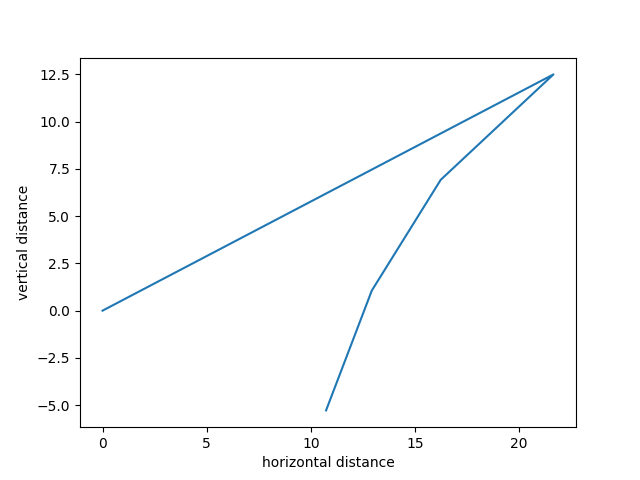
\includegraphics[width=\textwidth]{dtp5.png}
		\caption{$dt = 0.5s$ }
	\end{subfigure}
	\begin{subfigure}[h]{0.300\textwidth}
		\centering
		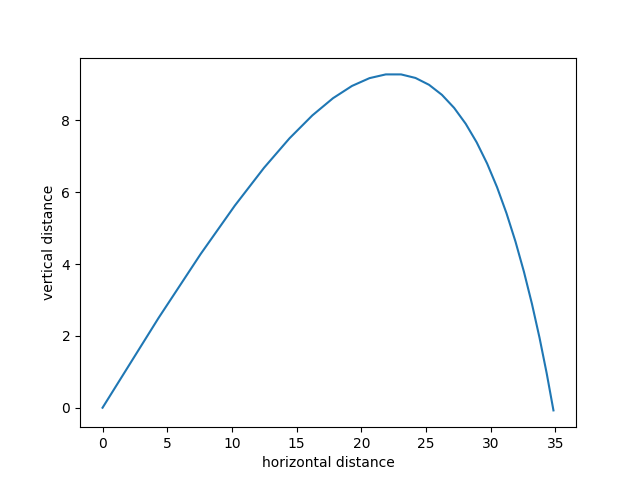
\includegraphics[width=\textwidth]{dtp1.png}
		\caption{$dt = 0.1s$}
	\end{subfigure}
		\begin{subfigure}[h]{0.30\textwidth}
		\centering
		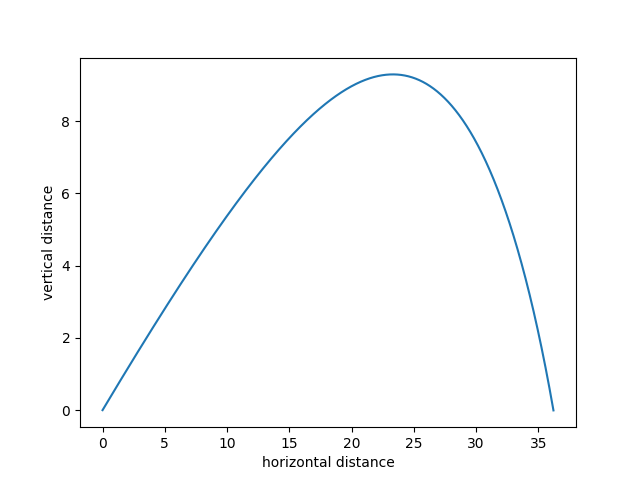
\includegraphics[width=\textwidth]{dt10e-2.png}
		\caption{$dt = 10^{-2}s$ }
	\end{subfigure}\\ 
	\begin{subfigure}[h]{0.30\textwidth}
		\centering
		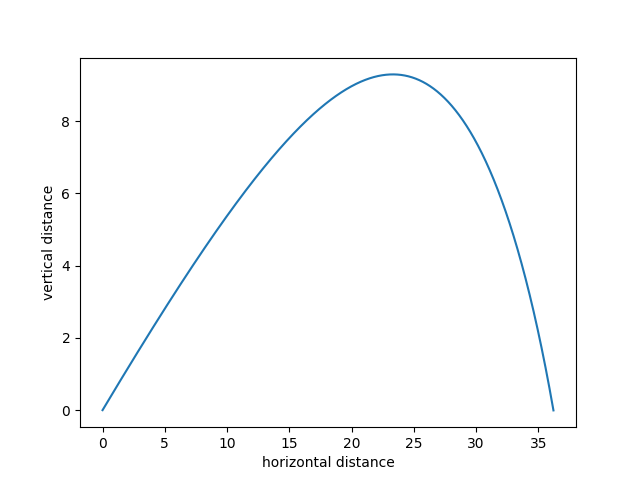
\includegraphics[width=\textwidth]{dt10e-3.png}
		\caption{$dt = 10^{-3}s$}
	\end{subfigure}
			\begin{subfigure}[h]{0.30\textwidth}
		\centering
		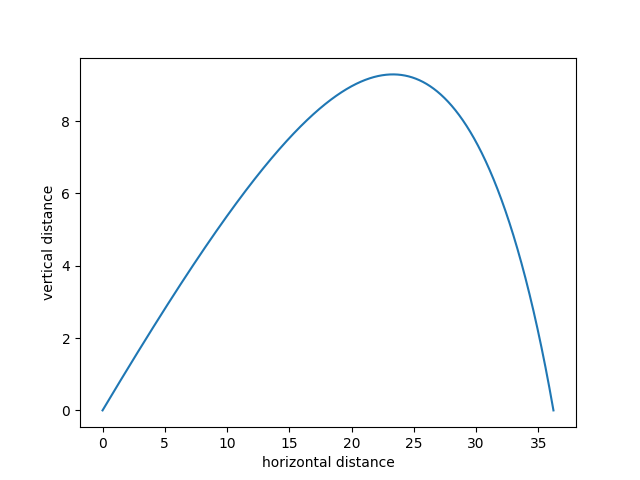
\includegraphics[width=\textwidth]{dt10e-4.png}
		\caption{$dt = 10^{-4}s$ }
	\end{subfigure}
	\begin{subfigure}[h]{0.30\textwidth}
		\centering
		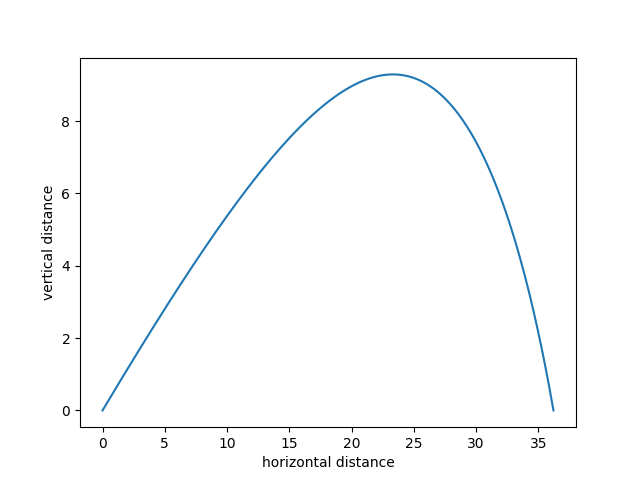
\includegraphics[width=\textwidth]{dt10e-6.png}
		\caption{$dt = 10^{-6}s$}
	\end{subfigure}
	\caption{Forward Euler - Finite difference}
\end{figure}
\\ It is clear that these plots fit the observation. The following results were obtained from each run as the ``Time of flight" and the ``Range" of the projectile.
\begin{center}
	\begin{tabular}{||c c c||} 
		\hline
		$dt$ & Range & Time of Flight \\ [0.5ex] 
		\hline\hline
		0.5 & 10.7329 & 2.5  \\ 
		\hline
		0.1 & 34.8447 & 2.7  \\
		\hline
		$10^{-2}$ & 36.1445 & 2.68  \\
		\hline
		$10^{-3}$ & 36.2110 & 2.669 \\
		\hline
		$10^{-4}$ & 36.2181 & 2.668 \\
		\hline
		$10^{-6}$ & 36.2191 & 2.667939 \\ [0.5ex]
		\hline
	\end{tabular}
\end{center}
It is easy to see that the method performs better with smaller time steps. Since it is an explicit method, it seems to be very unstable when $dt$ is large (notice that the time of flight is $\sim 2.5$s, and so, $0.5s$ is a pretty large time step). The most important take away is that - smaller time steps produce better results. However, depending upon the sensitivity of the problem, often times, we need not consider very small time steps. In this example, going from $dt = 10^{-4}$ to $dt = 10^{-6}$ is a hundred fold magnification, and yet still, the improvement of the output is only in the range of $10^{-4}$ - and more importantly, the average (over 10 runs) computation time when $dt = 10^{-4}$ was $0.002s$, however, the average (over 10 runs) computation time when $dt = 10^{-6}$ was $2.11s$; meaning computational cost of hundred fold magnification is about a thousand times large\footnote{Python's $timeit()$ module seems to be performing poorly from run to run, sometimes even returning negative values. So, I averaged the first ten positive outputs to produce a rough estimate. Once I figure out the technical details behind using the module, I would like to analyse the time and computational costs involved with smaller timesteps. Assuming that a computer can perform $10^6$ computations per second, I think that I would observe for $dt = 10^{-n}$, we would have computational time around $10^{n-6}$}.  This difference will only get bigger as we consider more complex problems. \\
\indent As sort of an extra personal project I also tried to impliment a slightly more stable explicit method for the same problem. For this I chose a $4^{th}$ order Runge Kutta method (because that was the one of the few stable methods in the notes that that related to coupled differential equations). With the help of a few online resources, I was able to impliment the method. I have attached my code for that in Appendix 1 as $4(b)$. The plots and results that I obtained from this method follow the same results produced by Forward Euler method. In what follows, I am assuming that the result obtained using Forward Euler is correct. \\
\begin{figure}[h]
	\centering
	\begin{subfigure}[h]{0.30\textwidth}
		\centering
		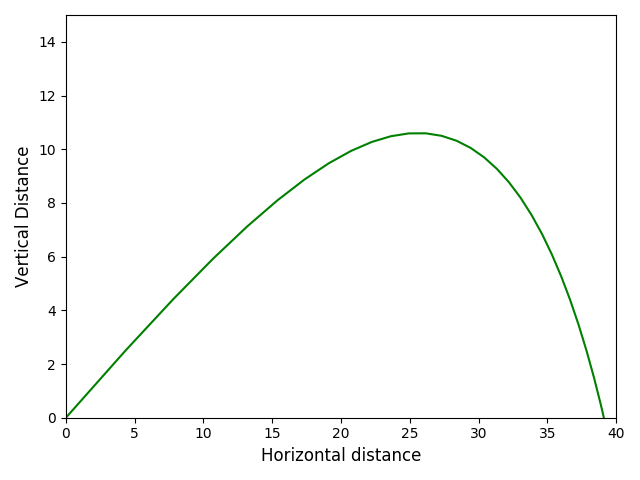
\includegraphics[width=\textwidth]{4orkdte-1.png}
		\caption{$dt = 0.1s$ }
	\end{subfigure}
	\begin{subfigure}[h]{0.300\textwidth}
		\centering
		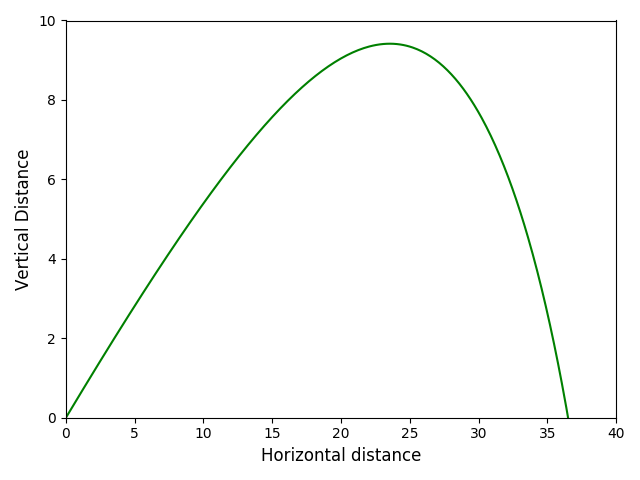
\includegraphics[width=\textwidth]{4ork.png}
		\caption{$dt = 0.01s$}
	\end{subfigure}
	\caption{Fourth Order Runge Kutta}
\end{figure}

\noindent The following are the results obtained from the $4^{th}$ order RK method. 
\begin{center}
	\begin{tabular}{||c c c||} 
		\hline
		$dt$ & Range & Time of Flight \\ [0.5ex] 
		\hline\hline
		0.1 & 38.8965 & 2.6  \\ 
		\hline
		$10^{-2}$ & 36.4735 & 2.68  \\
		\hline
	\end{tabular}
\end{center}
Surprisingly, the 4th order RK performs poorly by overestimating the result in both cases (in comparison to Forward Euler, that had a much faster convergence)\footnote{If we can assume the true result to be 36.2191, then when $dt = 0.1$, we have \\ $|36.2191 - 34.8447| < |36.2191 - 38.8965|$ and when $dt = 0.01$, we have $|36.2191 - 36.1445| < |36.2191 - 36.4735|$}. I believe this is the tradeoff between stability and accuracy. 

\newpage 
\begin{center}
APPENDIX 1 
\end{center}
\noindent \textbf{4(a)}\lstinputlisting[language=Python]{Hw6.py}


\newpage  
\noindent \textbf{4(b)}\lstinputlisting[language=Python]{rk4o.py}

\end{document}